\section{History}
\label{History}
\begin{NexMainBox}[light, hdrA, sdwA, grwB, crnA, title=\textbf{History of C}]
	\begin{NexMainBox}[dark, crnA]
		\begin{NexListDark}
			\NexItemDark{\NexFunction{1969 - B Language}: Word oriented (i.e. not byte oriented)}
			\NexItemDark{\NexFunction{1972 - Introduction of C}: Added multiple types, including byte and character types}
			\NexItemDark{\NexFunction{1972–1978 - Co-evolution of C and UNIX}: Reduced assembly language usage in UNIX}
			\NexItemDark{\NexFunction{1978 - K\&R C}: The first edition of "The C Programming Language" by Kernighan and Ritchie}
			\NexItemDark{\NexFunction{1989 - C89/ANSI}: ANSI standardization for C language}
			\NexItemDark{\NexFunction{1990 - C90/ISO C}: ISO standardization for C language}
			\NexItemDark{\NexFunction{1999 - C99}: Introduced features like complex types and Unicode support}
			\NexItemDark{\NexFunction{2011 - C11}: Focused on library improvements and added new functionalities}
			\NexItemDark{\NexFunction{2018 - C17}: Cleanup and minor features added}
		\end{NexListDark}
	\end{NexMainBox}
\end{NexMainBox}

\begin{NexMainBox}[light, hdrA, sdwA, grwB, crnA, title=\textbf{Language Tree}]
	\begin{NexMainBox}[dark, crnA, halign=center]
		\begin{tikzpicture}
			\tikzset{
				system/.style={
					rectangle,
					text=black,
					fill=yellow,
					rounded corners,
					text centered,
					font=\sffamily\bfseries
				},
				science/.style={
					rectangle,
					text=black,
					fill=green,
					rounded corners,
					text centered,
					font=\sffamily\bfseries
				},
				interpreted/.style={
					rectangle,
					text=white,
					fill=red,
					rounded corners,
					text centered,
					font=\sffamily\bfseries
				}
			}
			\node at (0,0) {
				\begin{tikzpicture}[
					sibling distance=2cm,
					level distance=0.69cm,
					anchor=north,
					grow=south,
					edge from parent path={
					(\tikzparentnode.south) .. controls +(0,-1) and +(0,1) .. (\tikzchildnode.north)
					}
				]
					\node[system](assembly){Assembly (1949)} child {
						child {
							node[science](fortran)[below=of assembly]{Fortran (1955)} child {
								node[system](c)[below=of fortran]{C (1972)} child {
									child {
										node[system](c++)[below=of c, anchor=north east]{C++ (1980)} child {
											node[system](csp)[below=of c++, anchor=north east]{C\# (1980)}
										}
									}
									child {
										node[system](objective-c)[below=of c, anchor=north west]{Objective-C (1980)} child {
											child {
												node[system](swift)[below=of objective-c, anchor=north west]{swift (1980)}
											}
										}
									}
									child {
										node[system](java)[above=of objective-c, anchor=north west]{java (1980)}
									}
									child {
										node[system](matlab)[left=of c++, anchor=south east]{MATLAB (1980)}
									}
								}
							}
						}
						child {
							node[system](cobol)[left=of fortran, anchor=south east]{COBOL ()}
						}
						child {
							node[system](lisp)[right=of fortran, anchor=south west]{LISP ()} child {
								child {
									node[system](haskell)[below=of lisp, anchor=north west]{Haskell (1980)}
								}
								child {
									node[system](r)[below=of lisp, anchor=north east]{R (1980)}
								}
							}
						}
					};
				\end{tikzpicture}
    			};
		\end{tikzpicture}
	\end{NexMainBox}
\end{NexMainBox}

\begin{comment}


	\draw (c) to node[midway, centered, white, ->] {}(php);
					\draw (c) to node[midway, centered, white, ->] {}(java);
					\draw (c) to node[midway, centered, white, ->] {}(python);
					\node at (8,6) {
						\begin{NexMainBox}[primary, coltwo]
							\begin{NexListDark}
								\NexItemDark{\textcolor{red}{\small{\textbf{Scripting/Interpreted}}}}
								\NexItemDark{\textcolor{yellow}{\small{\textbf{System}}}}
								\NexItemDark{\textcolor{green}{\small{\textbf{Science Calculations}}}}
							\end{NexListDark}
						\end{NexMainBox}


child {
							node[system](c) {C (72)} child {
								child {
									node[system] {C++ (80)} child {
										child {
											node[system] {C\# (01)}
										}
										child {
											node[system](java) {Java (95)}
										}
									}
								}
								child {
									node[system] at (5cm,0mm) {ObjectiveC (83)}
								}
								child {
									node[system] at (5cm,0mm)(javascript) {JavaScript (95)}
								}
								child {
									node[interpreted] at (0mm,0mm) {bash (79)} child {
										node[interpreted]  at (3mm,0mm) {perl (87)} child {
											child {
												node[interpreted](python) {python (91)}
											}
											child {
												node[interpreted](php) at (0.5cm,-10mm){php (95)}
											}
										}
									}
								}
							}



    \tikzset{
        directory/.style={
            text=white, % Text color
            fill=blue, % Fill color
            rounded corners, % Rounded edges
            text centered,
            font=\sffamily\bfseries
        },
        file/.style={
            text=white, % Text color
            fill=brown!60!black, % Fill color
            rounded corners, % Rounded edges
            text centered,
            font=\sffamily\bfseries
        },
        symlink/.style={
            text=white, % Text color
            fill=teal, % Fill color
            rounded corners, % Rounded edges
            text centered,
            font=\sffamily\bfseries
        }
    }

    \node at (0,0) {
        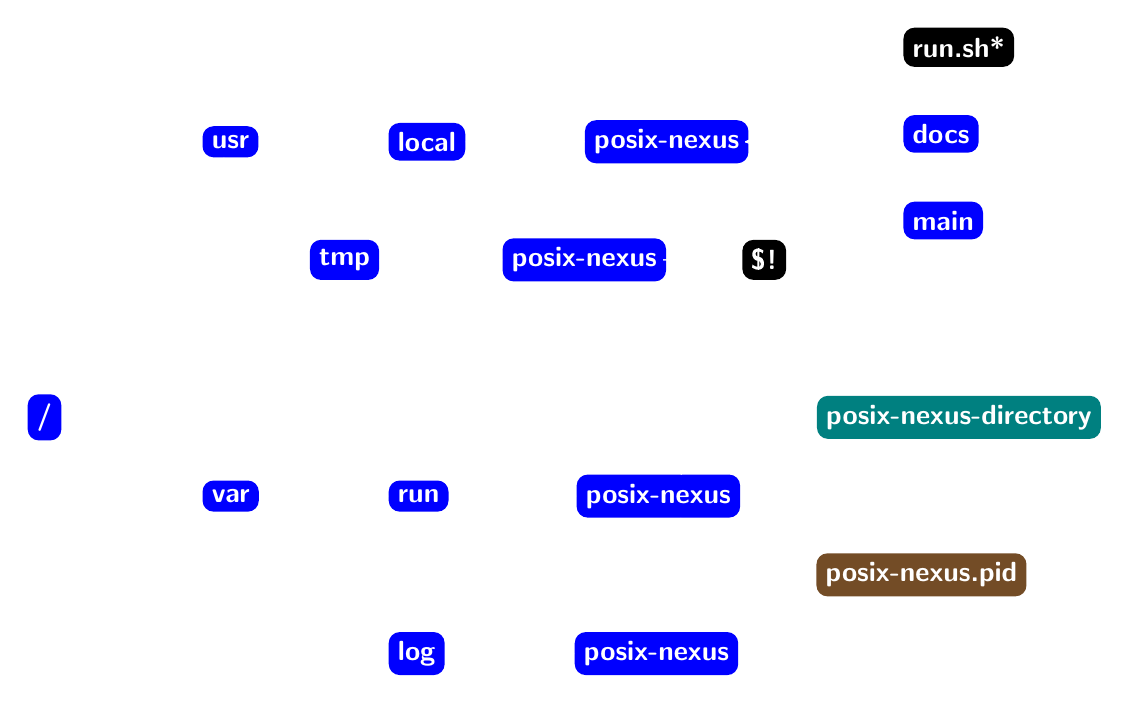
\begin{tikzpicture}[
            sibling distance=2cm,
            level distance=1cm,
            anchor=west,
            grow=east]
            \node[directory] {/} child {[white]
                child {node[directory]{var}
                    child {
                        child {node[directory]{log}
                            child {
                                child {node[directory]{posix-nexus}}
                            }
                        }
                        child {node[directory]{run}
                            child {
                                child {node[directory]{posix-nexus}
                                    child {
                                        child {node[file]{posix-nexus.pid}}
                                    }
                                    child[draw,dashed,thick] {
                                        child {node[symlink](b) at (0,0){posix-nexus-directory}}
                                    }
                                }
                            }
                        }
                        child {node[directory] at (-10mm,10mm){tmp}
                            child {
                                child {node[directory]{posix-nexus}
                                    child {
                                        child {node[directory,fill=black](a) at (0,0){\$!}}
                                    }
                                }
                            }
                        }
                    }
                }
                child {node[directory] at (0mm,25mm){usr}
                    child {
                        child {node[directory]{local}
                            child {
                                child {node[directory]{posix-nexus}
                                    child {
                                        child {node[directory] at (10mm,10mm){main}}
                                        child {node[directory] at (10mm,1mm){docs}}
                                        child {node[file,fill=black] at (10mm,-8mm){run.sh*}}
                                    }
                                }
                            }
                        }
                    }
                }
            };
            \draw[white,->] (b) to node[midway, centered, white] {\textbf{symlink}} (a);
        \end{tikzpicture}
    };
\end{tikzpicture}

\begin{NexCodeBox}{c}{title={if code is provides, put the code in me!}}
int main()
{
	printf("Im a minted box for C!!\n");
        return 0;
}
\end{NexCodeBox}
\end{comment}
